%
% FH Technikum Wien
% !TEX encoding = UTF-8 Unicode
%

\documentclass[MIC,Seminar,english]{twbook}%\documentclass[Bachelor,BMR,ngerman]{twbook}
\usepackage[utf8]{inputenc}
\usepackage[T1]{fontenc}
\usepackage[hybrid,pipeTables,tableCaptions]{markdown}
\usepackage{etaremune}

% for use in markdown:
\newcommand{\underscore}{\_}
\newcommand{\hash}{\#}
\newcommand{\n}{\\ \\}
\newcommand{\s}{\\}

% more useful commands:
% \noindent after ---
% \noindent\s after *
%
% Bitte in der folgenden Zeile den Zitierstandard festlegen
\newcommand{\FHTWCitationType}{IEEE} % IEEE oder HARVARD möglich - wenn Sie zwischen IEEE und HARVARD wechseln, bitte die temorären Dateien (aux, bbl, ...) löschen
%
\ifthenelse{\equal{\FHTWCitationType}{HARVARD}}{\usepackage{harvard}}{\usepackage{bibgerm}}

% Definition Code-Listings Formatierung:
\usepackage[final]{listings}
\lstset{captionpos=b, numberbychapter=false,caption=\lstname,frame=single, numbers=left, stepnumber=1, numbersep=2pt, xleftmargin=15pt, framexleftmargin=15pt, numberstyle=\tiny, tabsize=3, columns=fixed, basicstyle={\fontfamily{pcr}\selectfont\footnotesize}, keywordstyle=\bfseries, commentstyle={\color[gray]{0.33}\itshape}, stringstyle=\color[gray]{0.25}, breaklines, breakatwhitespace, breakautoindent}
\lstloadlanguages{[ANSI]C, C++, [gnu]make, gnuplot, Matlab}

%Formatieren des Quellcodeverzeichnisses
\makeatletter
% Setzen der Bezeichnungen für das Quellcodeverzeichnis/Abkürzungsverzeichnis in Abhängigkeit von der eingestellten Sprache
\providecommand\listacroname{}
\@ifclasswith{twbook}{english}
{%
    \renewcommand\lstlistingname{Code}
    \renewcommand\lstlistlistingname{List of Code}
    \renewcommand\listacroname{List of Abbreviations}
}{%
    \renewcommand\lstlistingname{Quellcode}
    \renewcommand\lstlistlistingname{Quellcodeverzeichnis}
    \renewcommand\listacroname{Abkürzungsverzeichnis}
}
% https://tex.stackexchange.com/questions/517657/annoying-syntax-highlighting-of-unclosed-group-at-csw
%%begin novalidate
% Wenn die Option listof=entryprefix gewählt wurde, Definition des Entyprefixes für das Quellcodeverzeichnis. Definition des Macros listoflolentryname analog zu listoflofentryname und listoflotentryname der KOMA-Klasse
\@ifclasswith{scrbook}{listof=entryprefix}
{%
    \newcommand\listoflolentryname\lstlistingname
}{%
}
%%end novalidate
\makeatother
\newcommand{\listofcode}{\phantomsection\lstlistoflistings}

% Die nachfolgenden Pakete stellen sonst nicht benötigte Features zur Verfügung
\usepackage{blindtext}

%
% Einträge für Deckblatt, Kurzfassung, etc.
%
\title{Reverse Engineering and Malware Analysis\\Assignments}
\author{Benjamin Medicke, BSc}
\studentnumber{2010303027}
%\author{Titel Vorname Name, Titel\and{}Titel Vorname Name, Titel}
%\studentnumber{XXXXXXXXXXXXXXX\and{}XXXXXXXXXXXXXXX}
\supervisor{Tibor Éliás, MSc.}
\secondsupervisor{Dipl.-Ing. Florian Nentwich}
%\supervisor[Begutachter]{Titel Vorname Name, Titel}
%\supervisor[Begutachterin]{Titel Vorname Name, Titel}
%\secondsupervisor{Titel Vorname Name, Titel}
%\secondsupervisor[Begutachter]{Titel Vorname Name, Titel}
%\secondsupervisor[Begutachterinnen]{Titel Vorname Name, Titel}
\place{Wien}

% TODO: ask if we need an outline:
%\kurzfassung{\blindtext}
%\schlagworte{Pentesting}
%\outline{\blindtext}
%\keywords{pentesting}

%\acknowledgements{\blindtext}

\begin{document}

%Festlegungen für den HARVARD-Zitierstandard
\ifthenelse{\equal{\FHTWCitationType}{HARVARD}}{
\bibliographystyle{Harvard_FHTW_MR}%Zitierstandard FH Technikum Wien, Studiengang Mechatronik/Robotik, Version 1.2e
\citationstyle{dcu}%Correct citation-style (Harvardand, ";" between citations, "," between author and year)
\citationmode{abbr}%use "et al." with first citation
\iflanguage{ngerman}{
    %Deutsch Neue Rechtschreibung
    \newcommand{\citepic}[1]{(Quelle: \protect\cite{#1})}%Zitat: Bild
    \newcommand{\citefig}[2]{(Quelle: \protect\cite{#1}, S. #2)}%Zitat: Bild aus Dokument
    \newcommand{\citefigm}[2]{(Quelle: modifiziert "ubernommen aus \protect\cite{#1}, S. #2)}%Zitat: modifiziertes Bild aus Dokument
    \newcommand{\citep}{\citeasnoun}%In-Line Zitiat entweder mit \citep{} oder \citeasnoun{}
    \newcommand{\acessedthrough}{Verf{\"u}gbar unter:}%Für URL-Angabe
    \newcommand{\acessedthroughp}{Verf{\"u}gbar bei:}%Für URL-Angabe (Geschützte Datenbank, Zugriff durch FH)
    \newcommand{\acessedat}{Zugang am}%Für URL-Datum-Angabe
    \newcommand{\singlepage}{S.}%Für Seitenangabe (einzelne Seite)
    \newcommand{\multiplepages}{S.}%Für Seitenangabe (mehrere Seiten)
    \newcommand{\chapternr}{K.}%Für Kapitelangabe
    \renewcommand{\harvardand}{\&}%Harvardand in Zitaten
    \newcommand{\abstractonly}{ausschließlich Abstract}
    \newcommand{\edition}{. Auflage}%Angabe der Auflage
}{
\iflanguage{german}{
    %Deutsch
    \newcommand{\citepic}[1]{(Quelle: \protect\cite{#1})}%Zitat: Bild
    \newcommand{\citefig}[2]{(Quelle: \protect\cite{#1}, S. #2)}%Zitat: Bild aus Dokument
    \newcommand{\citefigm}[2]{(Quelle: modifiziert "ubernommen aus \protect\cite{#1}, S. #2)}%Zitat: modifiziertes Bild aus Dokument
    \newcommand{\citep}{\citeasnoun}%In-Line Zitiat entweder mit \citep{} oder \citeasnoun{}
    \newcommand{\acessedthrough}{Verf{\"u}gbar unter:}%Für URL-Angabe
    \newcommand{\acessedthroughp}{Verf{\"u}gbar bei:}%Für URL-Angabe (Geschützte Datenbank, Zugriff durch FH)
    \newcommand{\acessedat}{Zugang am}%Für URL-Datum-Angabe
    \newcommand{\singlepage}{S.}%Für Seitenangabe (einzelne Seite)
    \newcommand{\multiplepages}{S.}%Für Seitenangabe (mehrere Seiten)
    \newcommand{\chapternr}{K.}%Für Kapitelangabe
    \renewcommand{\harvardand}{\&}%Harvardand in Zitaten
    \newcommand{\abstractonly}{ausschließlich Abstract}
    \newcommand{\edition}{. Auflage}%Angabe der Auflage
}{
    %Englisch
    \newcommand{\citepic}[1]{(Source: \protect\cite{#1})}%Zitat: Bild
    \newcommand{\citefig}[2]{(Source: \protect\cite{#1}, p. #2)}%Zitat: Bild aus Dokument
    \newcommand{\citefigm}[2]{(Source: taken with modification from \protect\cite{#1}, p. #2)}%Zitat: modifiziertes Bild aus Dokument
    \newcommand{\citep}{\citeasnoun}%In-Line Zitiat entweder mit \citep{} oder \citeasnoun{}
    \newcommand{\acessedthrough}{Available at:}%Für URL-Angabe
    \newcommand{\acessedthroughp}{Available through:}%Für URL-Angabe (Geschützte Datenbank, Zugriff durch FH)
    \newcommand{\acessedat}{Accessed}%Für URL-Datum-Angabe
    \newcommand{\singlepage}{p.}%Für Seitenangabe (einzelne Seite)
    \newcommand{\multiplepages}{pp.}%Für Seitenangabe (mehrere Seiten)
    \newcommand{\chapternr}{Ch.}%Für Kapitelangabe
    \renewcommand{\harvardand}{\&}%Harvardand in Zitaten
    \newcommand{\abstractonly}{Abstract only}
    \newcommand{\edition}{~edition}%Edition -> note, that you have to write "edition = {2nd},"!
}}}

\maketitle

%
% .. und hier beginnt die eigentliche Arbeit. Viel Erfolg beim Verfassen!
%

% group content by assignments:
\nocite{pracbin}

\begin{markdown}

# Reverse Engineering Exercise 1: Basics

**[Binary Provided: `2010303027_hw_1_exercise_1.exe`]**

## Calculate the value that the instruction at `0x40301B` loads into the RDI register!

* `lea rdi, ds:400FFEh[rcx*8] ; RDI = 0x????????????????`
* *note: the value in my example differs slightly*

\noindent\s To answer this question we need to know the value of `rcx`. I've extracted the relevant instructions with IDA: see Code \ref{excerpt1.1}.
\s

\end{markdown}
\begin{lstlisting}[language={[x86masm]Assembler},name={excerpt of relevant instructions task 1.1},label={excerpt1.1}]
.text:0000000000403014                 mov     rcx, 0Ah
.text:000000000040301B                 lea     rdi, ds:400FFBh[rcx*8]
\end{lstlisting}
\begin{markdown}

The mov instruction (line 1) copies the value `Ah` (`10`) into `rcx`. With that out of the way we can calculate the value with Python:

`hex(0x400ffb + 8 * 0xa)` which return `0x40104b` to us.
\n
This means that after executing the instruction (at least for the first time) the calculated value would be: **`40104Bh`**.
\n
Let's test that in IDA. We set a break point (*F2*) at the `lea` instruction and step over it (*F8*). As we can see in Figure \ref{calc} it is indeed correct.
\begin{figure}[!htbp]
\centering
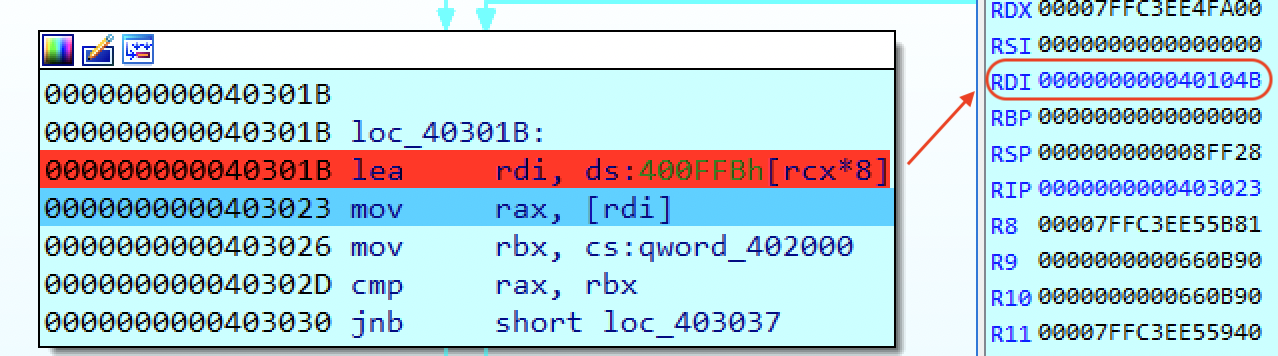
\includegraphics[width=.87\linewidth]{media/calc.png}
\caption{validating our calculation with IDA}\label{calc}
\end{figure}

## What is loaded into RAX when the instruction at address `0x403023` is run for the first time?

* `mov rax, qword[rdi] ; RAX = 0x????????????????`

\noindent\s
This builds on the previous example (the value of `rdi`). See Code \ref{excerpt1.2} for all relevant instructions.\s

\end{markdown}
\begin{lstlisting}[language={[x86masm]Assembler},name={excerpt of relevant instructions task 1.2},label={excerpt1.2}]
.text:0000000000403014           mov     rcx, 0Ah
.text:000000000040301B           lea     rdi, ds:400FFBh[rcx*8] ; rdi = 0x40104b
.text:0000000000403023           mov     rax, [rdi]
\end{lstlisting}
\begin{markdown}

The second `mov` instruction (line 3) copies the value that the address in `rdi` is pointing to into `rax`. Note the square brackets denoting dereferencing. Now all we need to know is where `0x40104b` points to.
\n
In IDA we can press *g* and jump to an address. We can either enter `0x40104b` or (if we're lazy and have stepped far enough) simply `rdi`. This leads us to to the data section (Code \ref{data1.2}).

\end{markdown}
\begin{lstlisting}[language={[x86masm]Assembler},name={excerpt of relevant data section task 1.2},label={data1.2}]
.data:000000000040104B db 0AFh
.data:000000000040104C db 0BEh
.data:000000000040104D db 0ADh
.data:000000000040104E db 0DEh
.data:000000000040104F db    0
.data:0000000000401050 db    0
.data:0000000000401051 db    0
.data:0000000000401052 db    0
\end{lstlisting}
\begin{markdown}

Reading it from the bottom up, our value is: **`DEADBEAFh`**, a classic.
\n
Same as before, let's make sure with IDA by stepping over it and taking a look at the register. Figure \ref{pred} shows us that we were correct.
\n
\begin{figure}[!htbp]
\centering
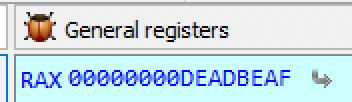
\includegraphics[width=.45\linewidth]{media/pred.png}
\caption{validating our prediction with IDA}\label{pred}
\end{figure}

\clearpage
## Is it possible that the application is defining an array of data somewhere in the program? If so what’s the address of the first element?

* Examine how the program access its data before you write the answer.

\noindent\s Let's get a rough overview of the program. IDAs graph view (*space*) is very useful for tasks like this. see Figure \ref{structure}, it starts right after the `scanf()` call and setting `rcx` to `10`.


\begin{figure}[!htbp]
\centering
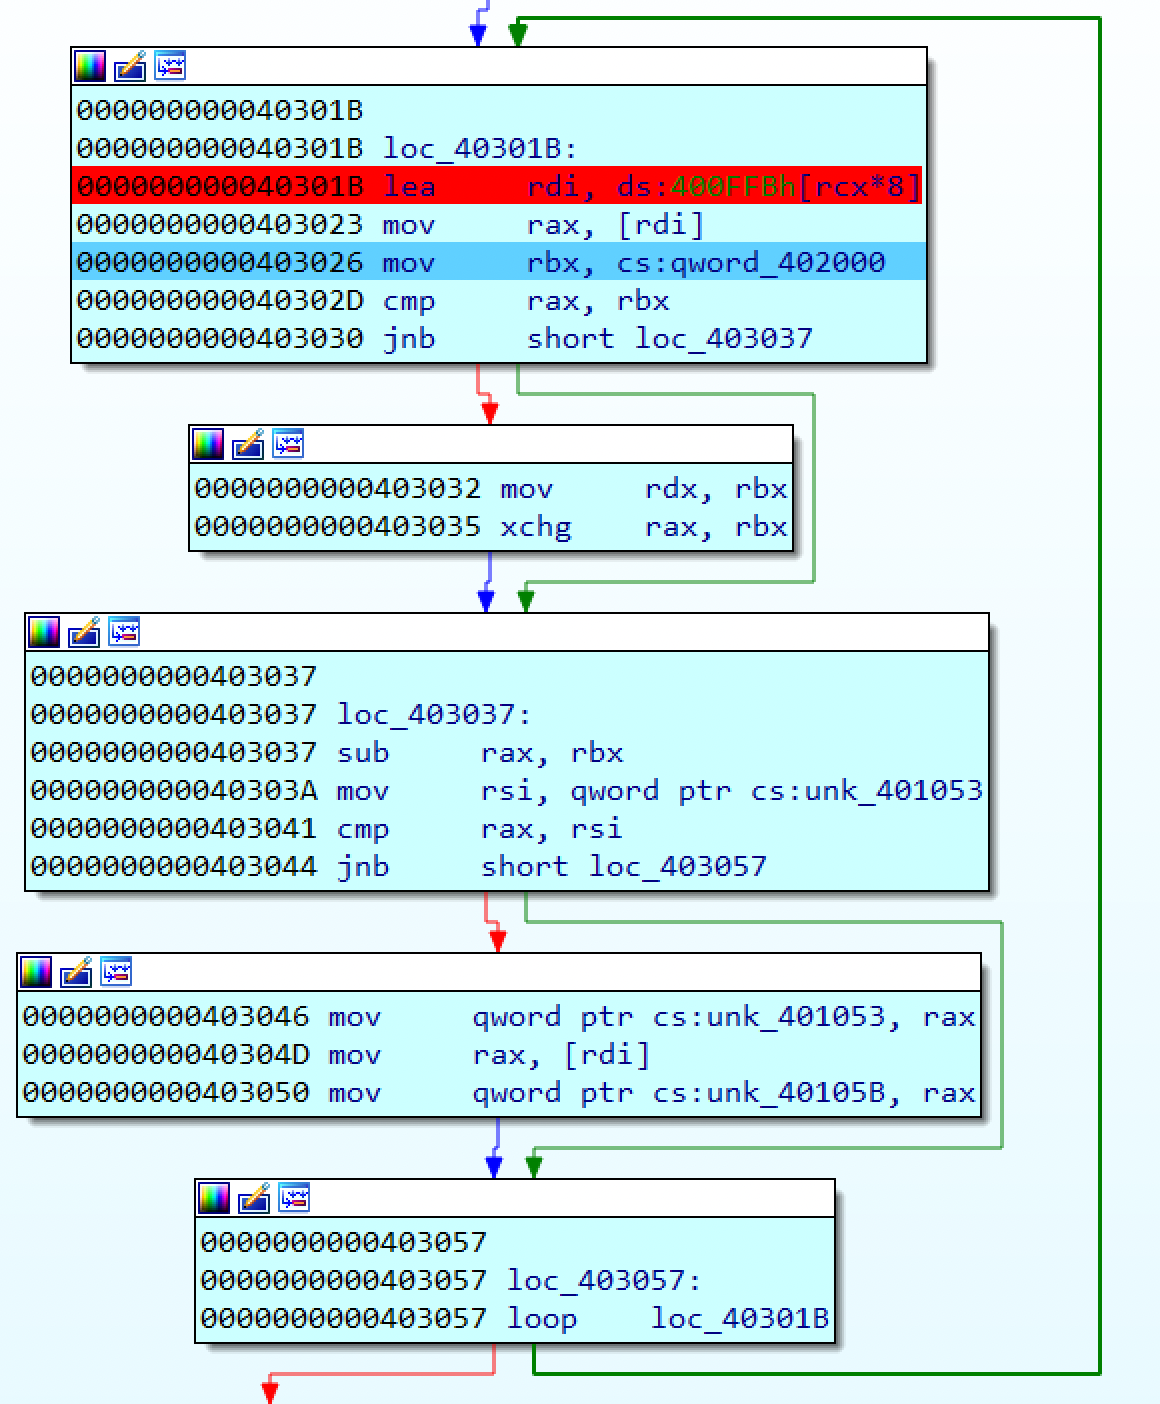
\includegraphics[width=.7\linewidth]{media/structure.png}
\caption{rough overview of the first program}\label{structure}
\end{figure}

\noindent The **first block** of code from `40301Bh` to `403030h` uses the value of the `rcx` register to calculate an address in the data section (notably in multiples of 8). As we have seen before the value of that address is subsequently loaded into the `rax` register.
\n
The **last block** of code (a single instruction) at `403057h` (conditionally) loops back to the first block. The `loop` instructions does the following:\s

* the counter register (`rcx`) is decremented by 1
* if the counter register is 0 the loop is terminated
* if not a jump is executed (in our case back to the first block) \cite{inteldev}

\noindent\s Let's take a look at the data section: jumping to `.data` puts us at the beginning of it, here we can find the format string.
\n
The array starts 4 byte after that (but is accessed in reverse order). After selecting the first element in IDA you can jump to the next element with *g* `+8` (and so forth).\s

\end{markdown}
\begin{lstlisting}[language={[x86masm]Assembler},name={beginning of array},label={data1.3}]
.data:0000000000401003 db '#',0 ; first element
.data:0000000000401005 db    0
.data:0000000000401006 db    0
.data:0000000000401007 db    0
.data:0000000000401008 db    0
.data:0000000000401009 db    0
.data:000000000040100A db    0
.data:000000000040100B db  75h ; second element
.data:000000000040100C db    0
.data:000000000040100D db    0
.data:000000000040100E db    0
; ...
\end{lstlisting}
\begin{markdown}

---

\noindent\s Here is how I came to that conclusion: the addresses (in the same order as accessed by the loop above) of all the elements of the array are the following -  via Python

`for rcx in range (10, 0, -1): print(hex(0x400ffb + rcx * 8))`

\begin{etaremune}
\item `0x40104b` (our `DEADBEAFh`)
\item `0x401043` (`433A34h`)
\item `0x40103b` (`2213h`)
\item `0x401033` (`5h`)
\item `0x40102b` (`100h`)
\item `0x401023` (`443h`)
\item `0x40101b` (`ABCh`)
\item `0x401013` (`111h`)
\item `0x40100b` (`75h`)
\item **`0x401003`** (`23h`)
\end{etaremune}

\noindent The counter variable starts at the bottom (`Ah` so `10` as a multiplier) and is subsequently decremented by 1. Since the loop is broken when `rcx` reaches zero the lowest `rcx` value to reach the instruction at `40301Bh` is `1`.
\n
The first element of the array is thus: `400FFBh + 1 * 8` which equals **`401003h`**. Each element has 8 Bytes (per the multiplier above).

## How many initialized global variables does this program define? 

Initialized global variables are located in the `.data` section. \cite{x64beg}. It starts at `0401000h` and ends at `402000h`.
\n
So far we have already encountered two:\s

* the format string starting at `401003h`
* the array starting at `401003h` (I'm going to count this as one)

\noindent\s They are joined by another two: quad-words at `401053h` and `40105Bh` (see Figure \ref{global})

\begin{figure}[!htbp]
\centering
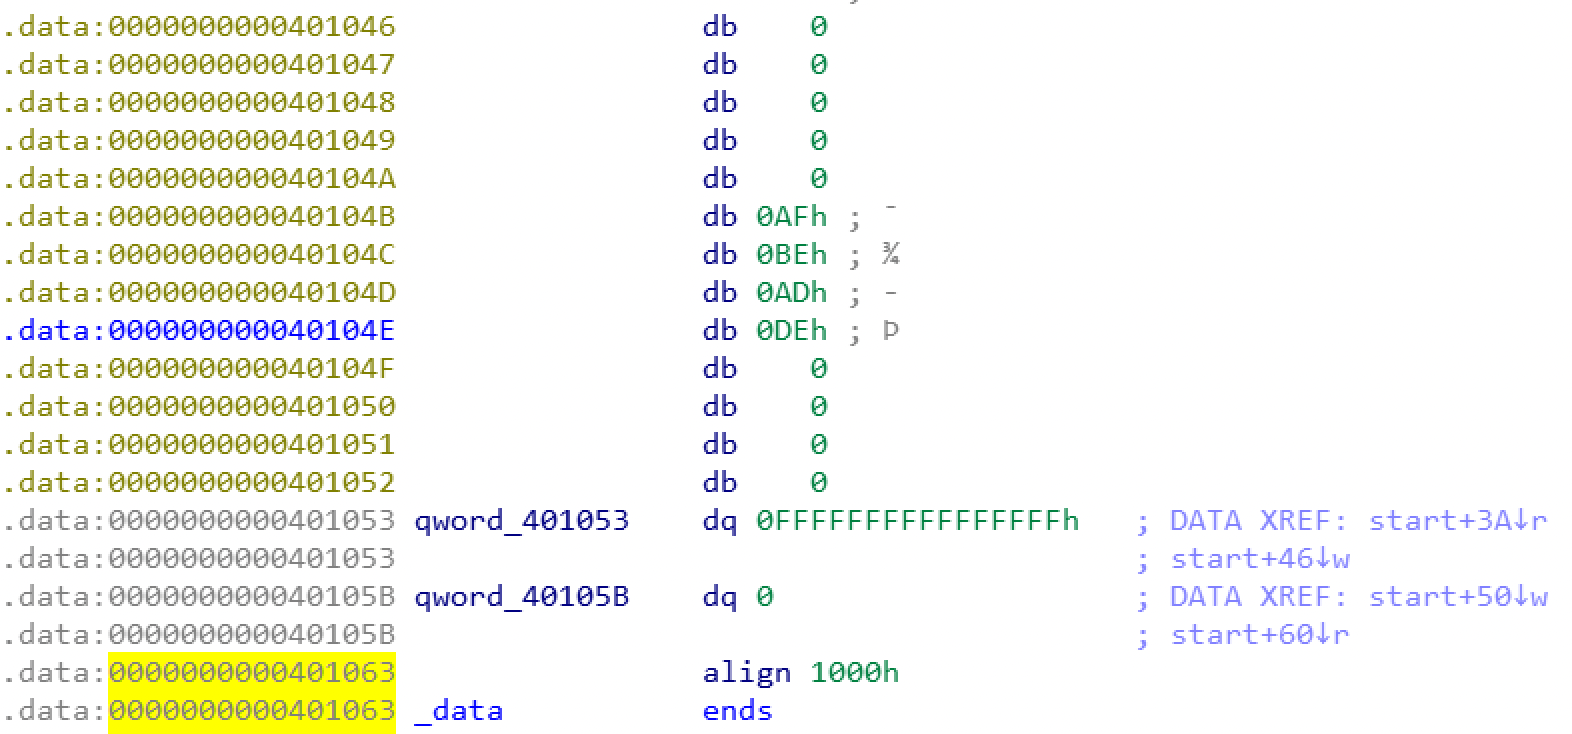
\includegraphics[width=1\linewidth]{media/global.png}
\caption{end of the array and the two quad-word (followed by no more discernible variables)}\label{global}
\end{figure}

\noindent The comment shows us where the two new quad-words are written and read from.

---

\noindent So **four** total.

## What happens if the value “433000” is passed to the program through the command line?

Passing the value `433000` to `2010303027_hw_1_exercise_1` results in the value `433A34` (see Figure \ref{433000}).

\begin{figure}[!htbp]
\centering
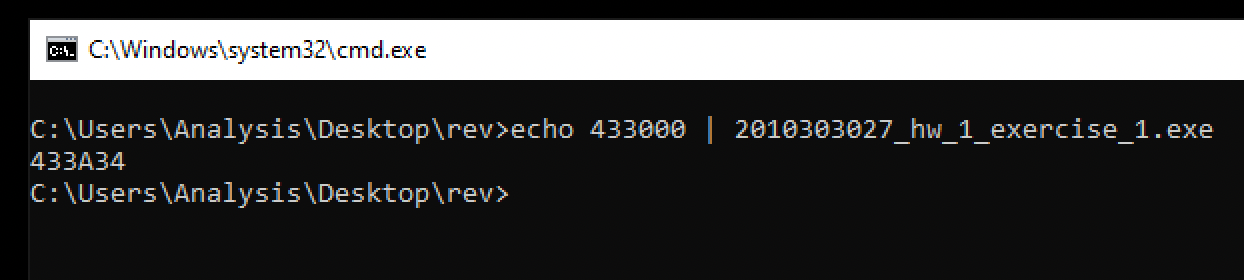
\includegraphics[width=\linewidth]{media/433000.png}
\caption{passing the value `433000` to `2010303027_hw_1_exercise_1.exe`}\label{433000}
\end{figure}

---

\noindent
I've also written a small Batch script that passes a range of values to possibly get a better understanding of the program without too much work: Code \ref{fuzzer}.
\newline
\end{markdown}
\begin{lstlisting}[language=command.com,name={fuzz.bat},label={fuzzer}]
@echo off
for /L %%G in (0, 1, 20000000) do (
  echo|set /p="%%G,  "
  echo %%G | C:\Users\ben\Desktop\2010303027\2010303027_hw_1_exercise_1.exe
  echo.
)
\end{lstlisting}
\begin{markdown}

Here is an excerpt of the output: Code \ref{log}.
\end{markdown}
\begin{lstlisting}[name={output via `fuzz.bat > log.txt`},label={log}]
0,  5
1,  5
# ...
13,  5
14,  5
15,  23
# ...
98,  75
99,  75
100,  111
101,  111
# ...
\end{lstlisting}
\begin{markdown}

It does give us a couple of input-value borders where the output value changes but is not particularly fast so I let it run in the background for a bit.
\n
Here is a list of values that I extracted from the log (on Linux via `sort -ut, -k2 log.txt`) before aborting the script. The left value is the first input value that results in a new output (right) value: \n

* 0,  5
* 15,  23
* 50,  75
* 100,  111
* 300,  443
* 780,  ABC
* 1000,  1000
* 1910,  2213
* 220000,  433A34

\noindent\s
Manually trying `-1` and random high values resulted in `DEADBEAF`, which are all (possibly) hex values. We already know all these values from our array!

\clearpage
## What does this program do? Describe it using your own words.

It reads input from the users and prints the closest value from an array.

---

\noindent Here's a more detailed outline (reference figure \ref{structure} for the loop):\s

* read **`user input`** as hexadecimal via `stdint` with `scanf()` (using format string `%X`)
* set **`counter`** register (`rcx`) to 10
* write **`user input`** to `402000h` in the `.bss` section (a quad-word)
* for each **`array element`** (from 10$^{th}$ to 1$^{st}$):
    * compare **`user input`** with **`array element`**:
        * if **`user input`** < **`array element`**: jump past switch
        * else: switch both values (simplifies the next step)
    * calculate absolute **`delta`**
    * compare **`delta`** with **`smallest known difference`** (that starts with max value):
        * if **`delta`** is lower update the **`smallest known difference`**
        * if **`delta`** is lower update the **`closest known element`**
    * decrement **`counter`**
* print the **`closest known element`** with `printf` (using the same format string)
* exit the program

\noindent\s The two quad-words we've seen in task 1.4 are used to store the `smallest known difference` (at `401053h`) and the `closest known element` (at `40105Bh`).

\clearpage
## Write a program that carries out the same task using any programming language you know
\end{markdown}
\begin{lstlisting}[language=python,name={finding the closest element with Python},label={python}]
#!/usr/bin/env python3

import sys


def get_closest_element():
    """
    this program prints the closest value from an array
    when compared with the userinput.
    """
    array = [
        0x23,
        0x75,
        0x111,
        0xABC,
        0x443,
        0x100,
        0x5,
        0x2213,
        0x433A34,
        0xDEADBEAF,
    ]

    user_input = int(input(), 16)
    smallest_difference = sys.maxsize
    closest_element = None

    # iterate through reversed array:
    for element in array[::-1]:
        # calculate current absolute delta.
        delta = abs(user_input - element)
        # update if we're closer:
        if delta < smallest_difference:
            smallest_difference = delta
            closest_element = element

    print(hex(closest_element))

if __name__ == "__main__":
    get_closest_element()
\end{lstlisting}
\begin{markdown}

\end{markdown}
\begin{markdown}

\clearpage
# Reverse Engineering Exercise 2: Crack me

**[Binary Provided: `2010303027_hw_1_exercise_2.exe`]**

## Fingerprint the program using any of the hashing tools that were presented during the lecture.

Here's a small report from HashMyfiles:\s

* Filename: `2010303027_hw_1_exercise_2.exe`
* MD5: `456809322ef371ca13c40b2626baa6a5`
* SHA1: `57fb1a64eb6099da090b063bd3e0e140f66cfa05`
* CRC32: `f6093492`

\noindent\s SHA-256: **`fc3a851c9958f5cafc9b04ffa4afae346c4633355e0d2d6f8a6b0f2292cef58e`**

## Run the program and enter an input value.

* What input value did you use? 

\noindent\s `123`

* What did you receive as an output?

\end{markdown}
\begin{lstlisting}[name={output pattern for input `123`}]
****
****
***:
*#*@
\end{lstlisting}
\begin{markdown}

---

\noindent\s I've continued to try values until I found the following pattern:

* `0`: `**`
* `1`: `*:`
* `2`: `*#`
* `3`: `*@`
* `4`: `:*`
* `5`: `::`
* etc. until `Fh` which is `@@`

\noindent\s These can be represented as Nibbles.

---

\noindent\s Assumption: break it down further:
`0` is `0b0000` so one `0b00` could represents a single `*`
If we compare it with `1` which is `0b0001` this could mean `:` is `0b0001`. Let's create a mapping and compare it with the values we know from our previous experiment.\s

* `00`: `*`
* `01`: `:`
* `10`: `#`
* `11`: `@`

\noindent\s This mapping checks out.

## What’s the address of the program’s entry point?

**`403000h`**

---

This is set in the PE header. In IDA you can load it by:\s

* loading the binary with the `Manual load` option
* answering yes to `Load the file header?` dialogue

\noindent\s Now you can jump to the header (*g* `HEADER:0`) and look for the address of the entry point.

\begin{figure}[!htbp]
\centering
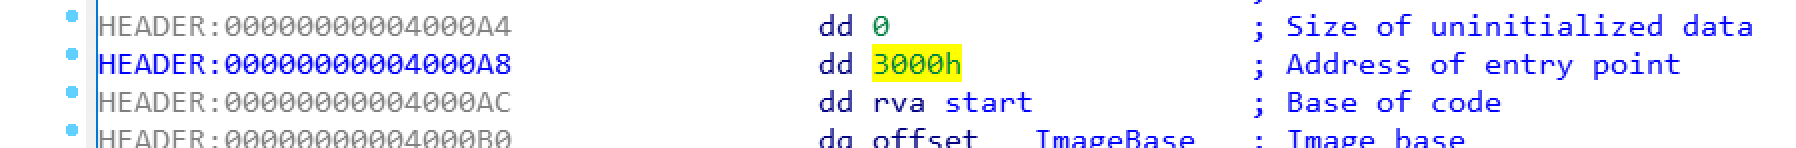
\includegraphics[width=\linewidth]{media/entry.png}
\caption{header of the }\label{entry}
\end{figure}

\noindent Adding this to the `image base` results in an address that is indeed the `start` of our program, see Figure \ref{entrypoint}.

\begin{figure}[!htbp]
\centering
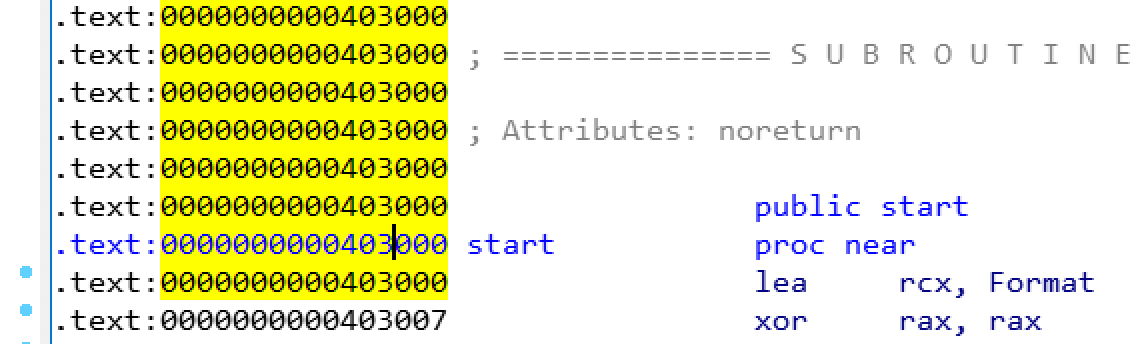
\includegraphics[width=\linewidth]{media/entrypoint.png}
\caption{the entry point of the second program}\label{entrypoint}
\end{figure}

\clearpage
## Identify the strings present in this program.

* Use one of the tools installed in the virtual analysis environment.

\noindent\s I'm really taking a shine to IDA so let's stick with that. There is a strings sub view, see Figure \ref{strings}.

\begin{figure}[!htbp]
\centering
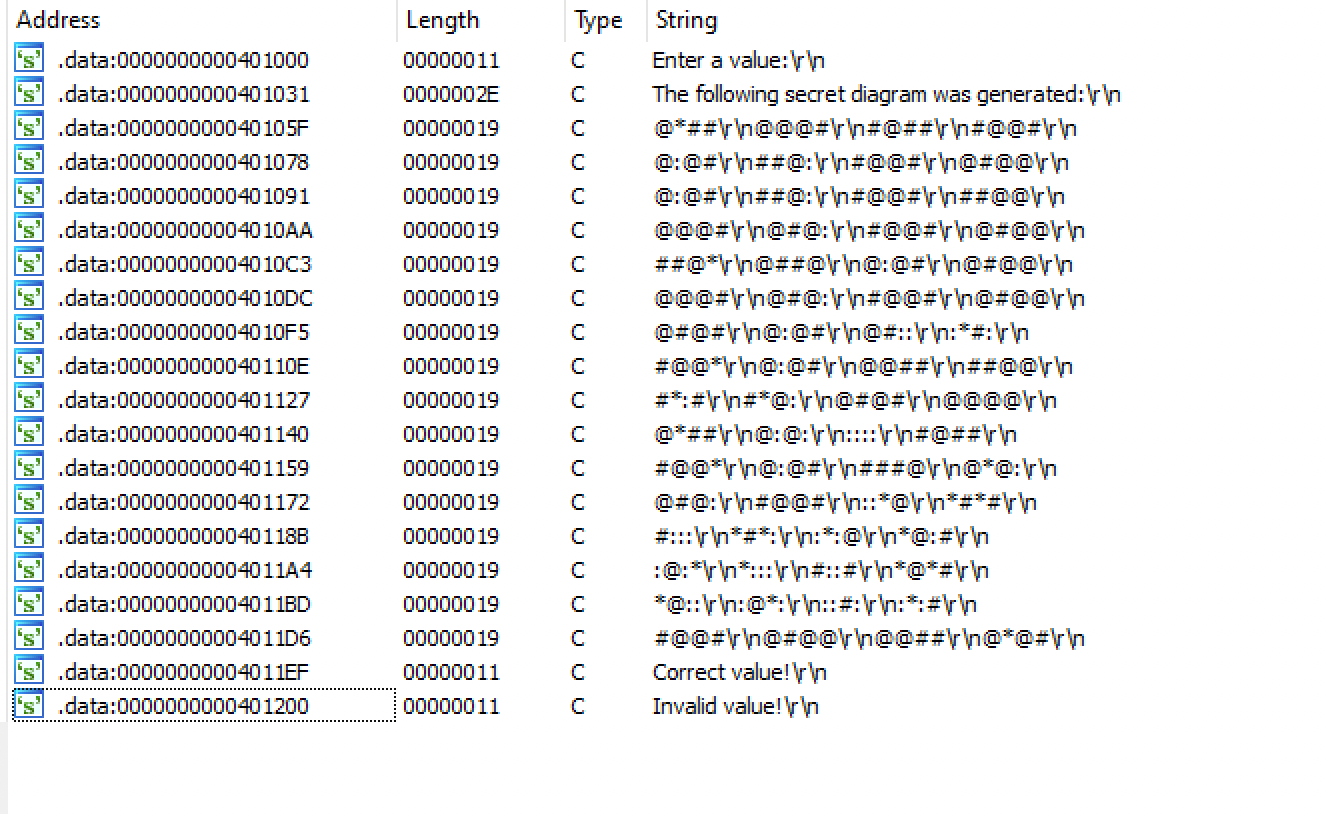
\includegraphics[width=\linewidth]{media/strings.png}
\caption{string sub view in IDA}\label{strings}
\end{figure}

There are a couple missing (like the DOS warning). Let's try it with `BinText`:\s

* load the binary
* include linefeed and carriage return in the `Filter` tab
    * to include strings from the secret diagram
* press `GO`

\end{markdown}
\begin{lstlisting}[name={more strings}]
00000000004D   0000C000008D      0   !This program cannot be run in DOS mode.
000000000188   000000000127      0   .data
0000000001D8   000000000177      0   .text
000000000200   00000000019F      0   .idata
# [...]
\end{lstlisting}
\begin{markdown}

Indeed a couple more that IDA hid from us!
## What sections are present in this program, what are their names and where are they located when the application is loaded into memory?

* Provide an address for each section

\noindent\s IDA provides a sub view for sections as well: see Figure \ref{sections}.\s

\begin{figure}[!htbp]
\centering
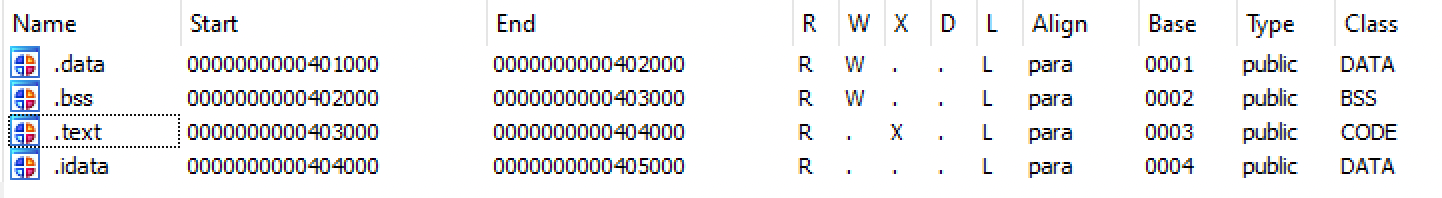
\includegraphics[width=\linewidth]{media/sections.png}
\caption{sections sub view in IDA}\label{sections}
\end{figure}

\noindent\s For the sake of readability, here are the section names and their respective start addresses:\s

* `.data`: `401000h`
* `.bss`: `402000h`
* `.text`: `403000h`
* `.idata`: `404000h`

## Identify all symbols that are imported by the program and their import directory (library)!

* Make sure you list all libraries that are linked to each import symbol and the address of each symbol
* Use a tool in the virtual analysis environment to make the search easier

\begin{figure}[!htbp]
\centering
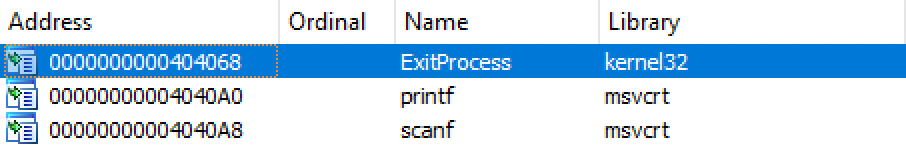
\includegraphics[width=\linewidth]{media/symbols.png}
\caption{imports sub view in IDA}\label{symbols}
\end{figure}

\clearpage
## Identify all exported symbols and their addresses

\begin{figure}[!htbp]
\centering
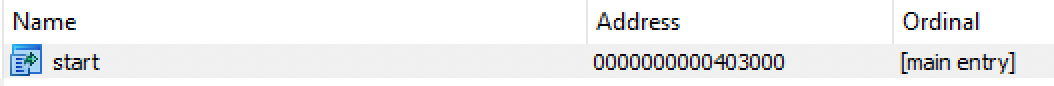
\includegraphics[width=\linewidth]{media/exports.png}
\caption{exports sub view in IDA}\label{export}
\end{figure}

## What calling convention is used by the following functions:

* `printf`
    * **x64 calling convention**
        * first parameter via `rcx`
        * similar to `__fastcall` but up to 4 instead of 2 registers
            * `rcx`, `rdx`, `r8`, `r9`
            * after that via the stack
* `scanf`
    * **x64 calling convention**
        * two parameters: `rcx` and `rdx`
* `sub_4030C7` (location `0x4030C7`)
    * **`__cdecl`**
        * cleaned up by caller (`add rsp, 10h`)
* `sub_403139` (location `0x403139`)
    * **`__stdcall`**
        * pushed to the stack: `401127h` and `402000h`
        * cleaned up by callee (`retn 10h`)
        
\begin{figure}[!htbp]
\centering
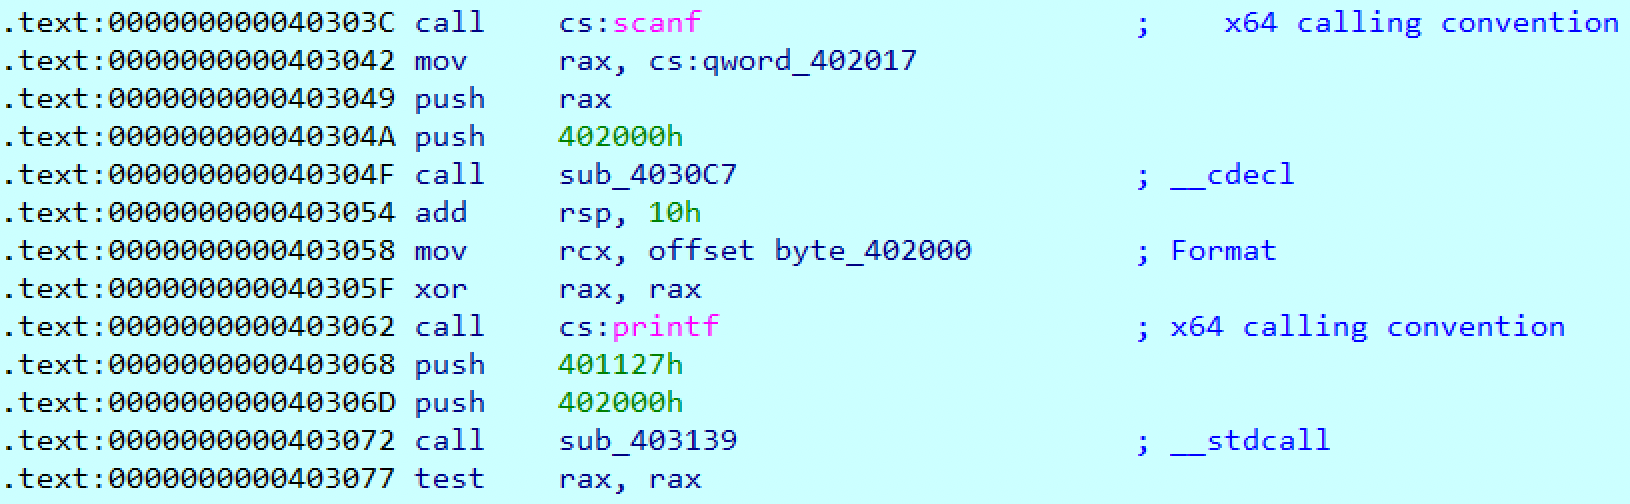
\includegraphics[width=\linewidth]{media/call.png}
\caption{calling conventions}\label{export}
\end{figure}

\noindent\s I've used Compile Explorer to play around with the different calling conventions with both x64 and x86 version of the `msvc` compiler: \href{https://godbolt.org/z/TcsToh}{https://godbolt.org/z/TcsToh}.

## Explain in your own words. What does this function do?

* `sub_4030A7` (location `0x4030A7`)

\noindent\s This function takes two bytes as input (via `rbx`) and returns a mapped character as an output (via `rax`).
\n
Possible input/output mappings:\s

* `00` -> `*`
* `01` -> `:`
* `10` -> `#`
* `11` -> `@`

---

\noindent Detailed order of operations (see figure \ref{a7}):
\n
\noindent This function is called in `sub_4030C7` via `.text:004030F5 call    sub_4030A7`. Before the call the following happens:\s

* `rbx` is nulled out everywhere but the 2 least significant bits (`and rbx, 3`)
* `rbx` is pushed to the stack as parameter for the call

\noindent\s If we assume that the user input is `ABCD1234`, the two least significant bits of `Ah` (`0b1010`) are `0b10`. This is the argument for the first time the function is called.
\n
In the function the following happens:\s

* `rbx` is pushed to the stack and popped to the lower `ebx`
* `rax` is set to `@` (`40h`, as a default value)
* the lowest byte of `ebx` is written written back, the upper filled with zeros
* `ebx` is compared with `0b11`:
    * if `ebx` is not bigger than `3`: use it as array lookup index and write value to `rax`
    * else: jump past array lookup (keeping the default value for `rax`)
* restore `ebp`
* exit

\noindent\s After the function the rest of the program can work with the return value (stored in `rax`).

\begin{figure}[!htbp]
\centering
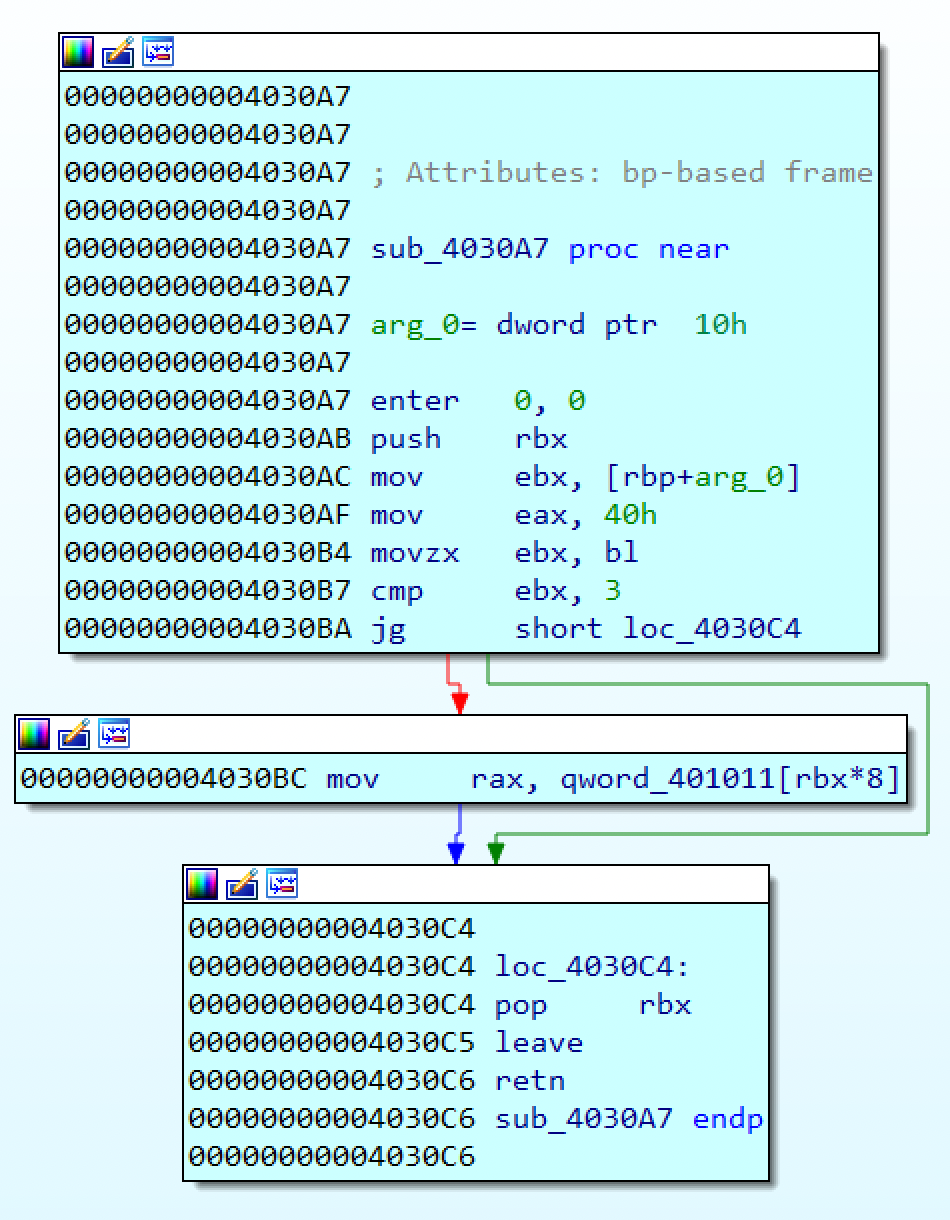
\includegraphics[width=0.8\linewidth]{media/a7.png}
\caption{the function `sub_4030A7`}\label{a7}
\end{figure}

## Figure out what code needs to be entered as an input in the console to match the diagram that is displayed. How did you find out?

* After the correct input has been provided, the following message should appear “Correct value!”

\noindent\s The pattern:

\end{markdown}
\begin{lstlisting}[name={target secret pattern}]
#*:#
#*@:
@#@#
@@@@
\end{lstlisting}
\begin{markdown}

Using the mapping from task 2.2 (plus the confirmation from task 2.9) and a bit of help from `calc.exe` we get: `868DEEFFh`. See Figure \ref{pattern} and Figure \ref{solution}.

\begin{figure}[!htbp]
\centering
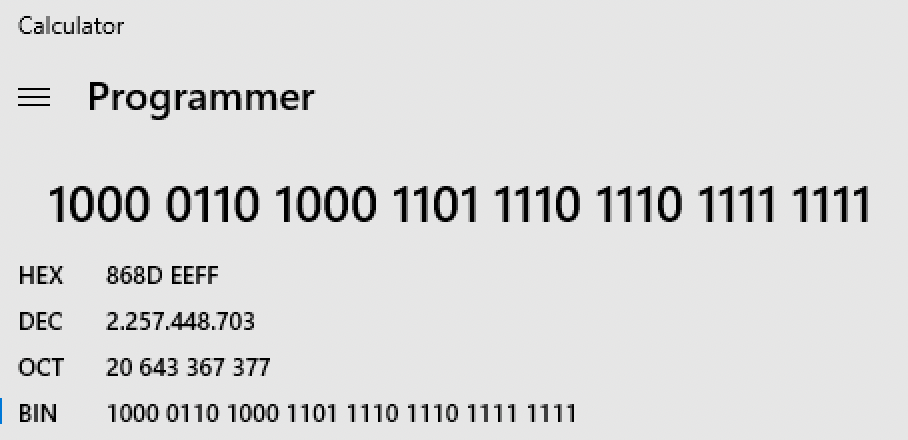
\includegraphics[width=\linewidth]{media/pattern.png}
\caption{converting the key from binary to hex}\label{pattern}
\end{figure}

\begin{figure}[!htbp]
\centering
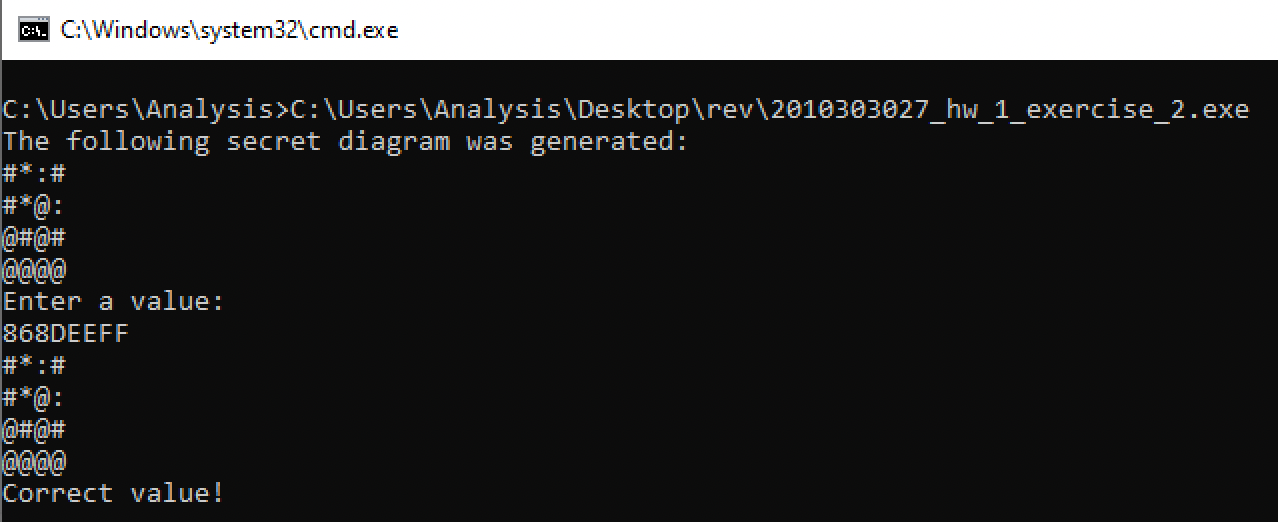
\includegraphics[width=1.1\linewidth]{media/solution.png}
\caption{checking the secret key}\label{solution}
\end{figure}

\end{markdown}
\clearpage
\begin{markdown}

% Die Virtual Box Detection selbst ist nicht gemeint, aber auf dem Weg dorthin wird vielleicht etwas gemacht, das die Analyse erschwert. ;-)

# Reverse Engineering Exercise 3: Malware Analysis

> \noindent Imagine you are an analyst in an anti-virus company and given the malware sample in the archive. Users report
> that they get blackmailed to transfer some amount of bitcoins to an evil person, otherwise access to the files
> will be denied forever.
\s
> Here is some useful information:

* The main function of this program starts at `0x4013F4`. This is the perfect starting point for your debugging session (i.e. set a breakpoint at that location with your favorite debugger).
* This executable does actually encrypt files on the disk. So please execute with care and take a snapshot before working on it

## Anti-Analysis Protection

> \noindent The piece of malware has anti-analysis protection. What is done to prevent malicious code execution in your VirtualBox environment? Please explain in detail and describe how you bypassed the check.

\noindent The binary tries to detect whether it is called from within Virtual Box by checking for a DLL that ships with the Virtual Box Guest Additions: 
`C:\windows\syswow64\vboxnine-x86.dll`.

\noindent\s See Figure \ref{vbox_check}. This code does the following:

* load `Shlwapi.dll` via `LoadLibraryA` so we can use its `PathFileExistsA`
* use `PathFileExistsA` to check for `C:\windows\syswow64\vboxnine-x86.dll`
    * it returns `true` if the file exists
    * it returns `false` if not
* if it does not exist jump past setting `byte_405638` to `1` and calling `sub_4012C4`
    * the variable keeps track of if we are in a VM/debugger
    * the subroutine is used to generate an exception in the debugger
        * by trying to write to `0x0` in a new thread (See Code \ref{crash_code}.)
            * jumping to `mov byte ptr [r14], 1` while `r14` points to `0x0`
            * which is written in to the process memory of the thread
            * which throws the exception when created
        * this code is reused by all the other checks (as a consequence)
* so **if we are in a VM (the file exists) the crash code is executed** to stop further analysis

\end{markdown}
\begin{figure}[!htbp]
\centering
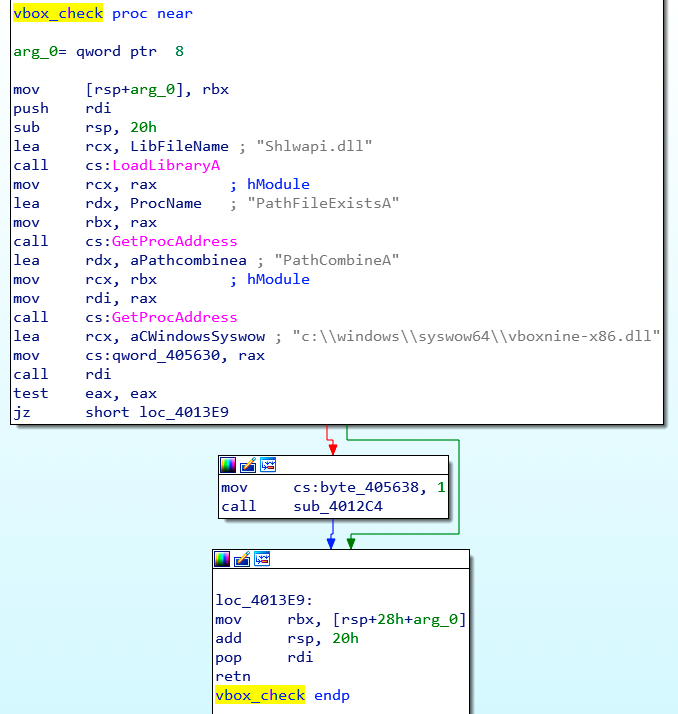
\includegraphics[width=\linewidth]{media/vbox_check.png}
\caption{the check that looks for the VBox DLL}\label{vbox_check}
\end{figure}
\begin{markdown}

\end{markdown}
\begin{figure}[!htbp]
\centering
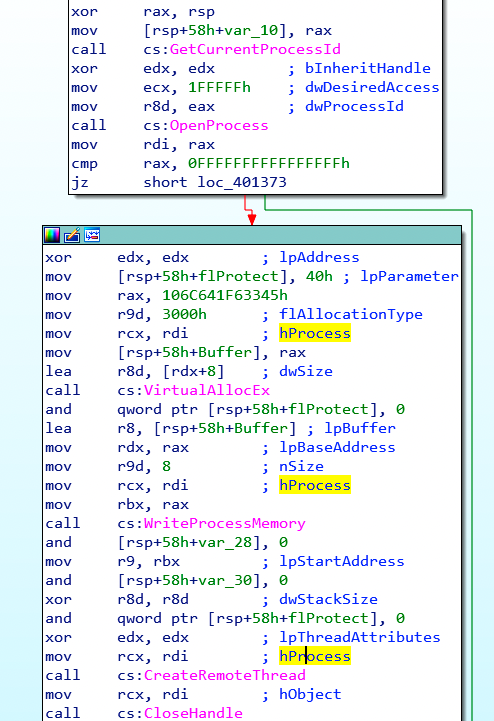
\includegraphics[width=\linewidth]{media/crash_code.png}
\caption{the code that ultimately throws an exception}\label{crash_code}
\end{figure}
\begin{markdown}

\clearpage
To bypass this (and other) checks we have a couple of options, among them:\s

* dirty hack: uninstall the Guest Additions or delete/rename the DLL 
* patch: change the string to a non-existing file
* patch: change the conditional jump for this check
* register manipulation: keep changing the zero flag to get past the crash code
* patch: **jump past the exception code in `sub_4012C4`** (the crash code)
    * this allows us to work around all checks with a single patch
    * the checks will still trigger but they won't throw an exception
    * I've chosen this option
    
---

\noindent I've patched the instruction at `0x4012FA` from `je 0x401373` to `jmp 0x401373`.
This effectively **always** jumps past the crash code allowing us to use the binary both inside and outside a VM and/or debugger.
\n
I think this is a rather clean solution but I've also mentioned possible other patches for all further checks.

---

\noindent Here is a binary diff via Radare2 that shows the entirety of the patch I've ended up with: Code \ref{radiff}.\n

\end{markdown}
\begin{lstlisting}[language=bash,name={binary diff},label={radiff}]
ben::cyric:shared:$ radiff2 -D Crypter_A.exe Crypter_A_betterpatch.exe
--- 0x000006fa  74
- je 0x79
- xor edx, edx
+++ 0x000006fa  eb
+ jmp 0x7b
+ xor edx, edx
\end{lstlisting}
\begin{markdown}

## Three More Protections Against Analysis

> \noindent Find three other ways that the executable tries to protect itself from manual analysis. Please explain them in detail and describe how you bypassed the protection measures.

* **delta time check** via `GetTickCount64()`s
    * this check actually starts before the check from the previous task
        * the current tick count is saved (`0x401409` and `0x40140`)
        * the first check is executed (`0x401412`)
        * the current tick count is saved again (`0x401417`)
        * the delta of the two counts is calculated and compared with 1000 ms (`0x40141D` to `0x401431`)
    * if it took longer (as when carefully stepping through the program) the check triggers
    * if you don't manually step through the program you don't have to patch this at all (it will only trigger if you take more than 1 second between the two calls to `GetTickCount64()`)
    * possible patch: increase the 1000 ms (`0x3E8`) to a higher value or patch the jump
* **`CheckRemoteDebuggerPresent()`**
    * called at `0x401455`
    * this checks if the process is attached to a debugger
    * the return value is tested for zero `0x40145B`
    * `0x40145D` jumps if it was non-zero (to the aforementioned crash code)
    * in conclusion: crash if the process is attached to a debugger
    * possible patch: nop out the call (`rax` is zero before it)
* I'm not sure what I would classify as the third additional countermeasure. Maybe the usage of the variable **`byte_405638`** to keep track of the outcome of the checks. All these checks are made inconsequential by my crash code patch.
Maybe stack cookies? But those are not really a hindrance since we're not writing a buffer overflow and have full control over them (and they are more of a compiler feature anyway). 
Or the `IsProcessorFeaturePresent` fastfail-check before the main (but that never gets executed and does not prevent analysis). Some dead code? I did not find a noticeable amount that would prevent analysis.
* Or maybe it's the fact that there is no Bitcoin address in sight, even though people are supposed to send some to get the key. That would certainly stump me as an analyst ;)
* I've spent so much time thinking about what the third protection mechanism might be; maybe it's the task itself. Very meta.

## Persistence

> \noindent Does the executable make itself persistent in the system? If so, please explain how.

\noindent There seems to be no persistence.

---

\noindent I could not find any persistence, neither by looking in the binary nor by fetching all processes with `tasklist` and diffing them with a known clean state.
I've also checked in the common places (registry, etc.) without avail.
\n
The binary does not seem to be set up for persistence either (e.g. by looking for new files and encrypting them as they are added).
Simply running the encryption on startup again would not make any sense either, since the encryption function is its own inverse function.

## Which Files Are Encrypted?

> Which files are encrypted? Please explain how you figured that out.

\noindent All the Python (`.py`) files in the `C:\Tools` folder. (Incidentally the file type I would least want to lose in a ransomware attack.)

---

\noindent I have figured this out early on since I usually take a look at all strings in a binary as one of the first steps. Here the globbing pattern and the path caught my eye. See Figure \ref{dstrings}.

\begin{figure}[!htbp]
\centering
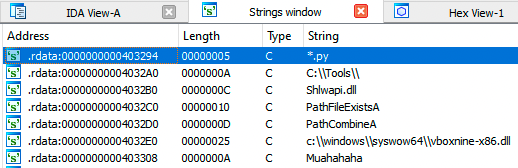
\includegraphics[width=\linewidth]{media/dstrings.png}
\caption{partial list of strings in malware}\label{dstrings}
\end{figure}

\noindent Looking for the occurrences of these two strings (via xrefs) quickly lead me to the piece of code that iterates over all files and directories in `C:\Tools` and the extension check (for Python files), which confirmed my suspicion. See Figure \ref{xrefs}.

\begin{figure}[!htbp]
\centering
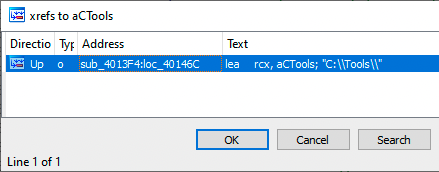
\includegraphics[width=\linewidth]{media/xrefs.png}
\caption{cross references for the `C:\Tools` variable}\label{xrefs}
\end{figure}

\noindent After patching the binary and running it I had further confirmations since all Python files in the Tools directory were indeed encrypted (and decrypted if run again).

## Parameters for `CreateFileA`

> \noindent There are two different calls to CreateFileA. Besides the filename parameter, please explain the parameters given to those two calls (value and meaning in your own words).

* the first call at `0x4010BB`
    * a pointer to the string of a python filename as `lpFileName`
    * `0x80000000` for `dwDesiredAccess`: **`GENERIC_READ`**
        * get read access to resource (Python file in our case)
        * to read the content (so it can xor/encrypt it)
    * `0x3` for `dwShareMode`: **`FILE_SHARE_READ`** plus **`FILE_SHARE_WRITE`**
        * to allow both read and write access rights to the file by other processes
    * `0x0` for `lpSecurityAttributes`, so **`NULL`**
        * the file handle can't be passed to a child processes
        * and the file gets a default security descriptor
    * `0x3` for `dwCreationDisposition` **`OPEN_EXISTING`**
        * this mode will throw an error if the file does not exist as opposed to silently creating it (**`ERROR_FILE_NOT_FOUND`**)
    * `0x8000000` for `dwFlagsAndAttributes`: **`FILE_FLAG_SEQUENTIAL_SCAN`**
        * used for sequential file access from beginning to end
        * this is used as a hint to Windows which helps it with optimizing caching behaviour
            * for example: no need to keep already read content in cache (because we're only moving forward)
    * for `hTemplateFile`
        * this is ignored because we're opening an existing file
    * if everything went allright we have a read handle now
* the second call at `0x4010F3`
    * this is executed if we got a valid (read) file handle from the previous call
    * same filename as the call preceding it
    * `0x40000000` for `dwDesiredAccess`: **`GENERIC_WRITE`**
        * now the malware actually wants to write the encrypted content
    * all the other parameters are the same as for the previous call
    * if everything worked we now have a valid write handle as well

## The Encryption Method

> \noindent Which encryption method is used? Please explain the piece of code responsible for it.

\noindent **The encryption method boils down to a bytewise XOR.**

---

\noindent The program iterates through all files and folders (skipping the current folder `.` and the parent folder `..`) looking for all python files along the way.  If one is found the absolute path to that file is concatenated and the address that points to that string is loaded into `rcx`. 
\n
Before the real encryption starts a bit of preparation happens, starting at `0x401000`:\s

* the encryption key is calculated and stored in `rsi` (see next section)
* a read and write handle is created (see previous section)

\noindent\s Now a single byte is read (at `0x40114B`).
\n 
\noindent **This single byte is `xor`ed with the calculated key at `0x40110E`:\s `xor     [rsp+160h+var_120], sil`**.
\n
This new encrypted byte is written back (in place) to the file at `0x40112C`:\s
`call    cs:WriteFile`.
\n
This repeats until the entire file is encrypted (and thus no more bytes can be read).
## The Encryption Key

> \noindent What's the encryption key being used for encryption? How is it calculated? 

The encryption key is 68, which is `0x44` or `0b1000100`.

---

\noindent The key is based on the username of the executing user which is fetched  via `call cs:GetUserNameA`.
\n
The following is an algorithm of how it is derived:\s

* get the username: `Analysis` (at `0x401040`)
* count chars in username string: `8` (1-indexed, `0x40104F` to `0x401055`)
    * by `inc`ing until we hit the string terminator
* add up all individual ASCII values (using our counter, `0x401064` to `0x401075`):
    * A: `0x41`
    * n: `0x6E`
    * a: `0x61`
    * l: `0x6C`
    * y: `0x79`
    * s: `0x73`
    * i: `0x69`
    * s: `0x73`
* which totals `0x344` in our case
* `AND` this value with `0x800000FF` (mask out, at `0x401077`)
    * keep only the leftmost (sign) and the 8 rightmost bits
* which gives us `0x44` our key!

---

The same in Python:

\end{markdown}
\begin{lstlisting}[language=python,name={key_calculator.py},label={keycalc}]
sum = 0
for c in 'Analysis': sum += ord(c)
hex(sum & 0x800000FF)  # '0x44'
\end{lstlisting}
\begin{markdown}

## Writing a Decryptor

> \noindent Share some piece of pseudo-code for a decryption tool that could be distributed to customers.

\noindent I've opted for Python instead of pseudo-code so I could test it and make sure not to forget any steps (plus it's fun to write). I've used Python 2 instead of 3 because that's the one that was available on the Windows box. See Code \ref{decryptor}. \n
This piece of code assumes that the customer has created a backup before running the decryptor in case anything goes wrong (and we want to build that habit for the future).

\end{markdown}
\begin{lstlisting}[language=python,name={decryptor.py},label={decryptor}]
#!/usr/bin/env python2
import os

path = 'C:\Tools'
filetype = '.py'
key = 0x44


def decrypt(filename):
    print 'decrypting ', filename
    decrypted = ''

    # read and decrypt content of file:
    with open(filename, 'rb') as file:
        for byte in file.read():
            decrypted += chr(ord(byte) ^ key)  # xor each byte with key.

    # write back decrypted content:
    with open(filename, 'wb') as file:
        file.writelines(decrypted)


# recursively iterate through path:
for subdir, dirs, files in os.walk(path):
    for filename in files:

        # decrypt affected files:
        if filename.endswith(filetype):
            decrypt(subdir + os.sep + filename)
\end{lstlisting}

%\begin{markdown}

\end{markdown}
%\begin{markdown}

\end{markdown}

% markdown and latex formatting examples:
%\begin{markdown}

# Start: example\underscore md.tex

Das \ac{ABC} ist *toll* und **praktisch**.

* das ist eine
* Liste
    * mit
    * Unterliste

---

horizontal rulers work

> das ist ein blockquote
>
> mit break

## Chapter 1.1

lorem ipsum
\newline
\end{markdown} % lstlistings don't work properly from within markdown!
\begin{lstlisting}[language=sh,name={checking Nmap's version},label={sc:nmapversion}]
root::kali:MCS_WH1:# nmap -V | head -n1
Nmap version 7.91 ( https://nmap.org )
\end{lstlisting}
\begin{markdown}

lorem ipsum

\begin{figure}[!htbp]
\centering
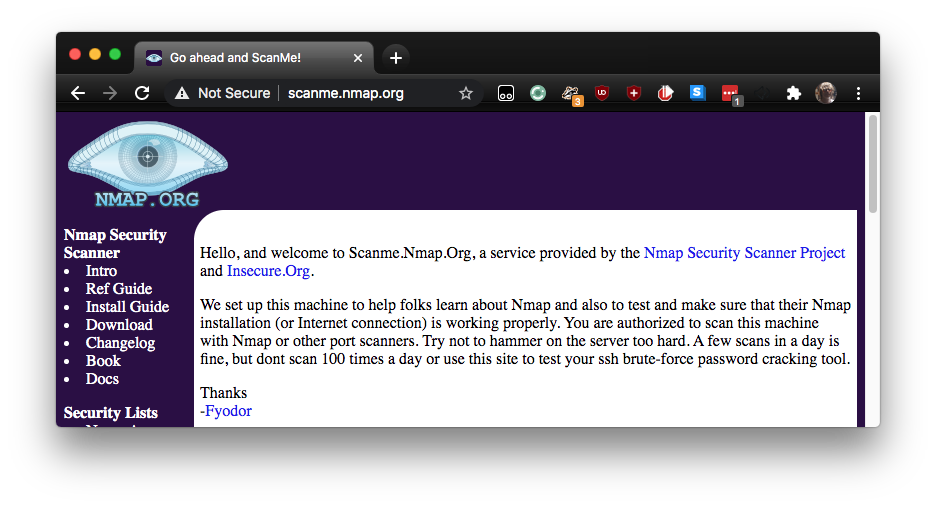
\includegraphics[width=1.05\linewidth]{media/scanme.nmap.org.png}
\caption{web server running at scanme.nmap.org}\label{webserver}
\end{figure}

Images work as well. See Figure \ref{sc:zahlenraten2}.
\newline
\end{markdown} % lstlistings don't work properly from within markdown!
\begin{lstlisting}[language={[x86masm]Assembler},name={disassembly of `zahlenraten`},label={sc:zahlenraten2}]
; ...
   0x0040077e <+14>:    56                  push   esi
   0x0040077f <+15>:    53                  push   ebx
   0x00400780 <+16>:    51                  push   ecx
=> 0x00400781 <+17>:    81 ec 08 02 00 00   sub    esp,0x2088
; ...
\end{lstlisting}
\begin{markdown}

Assembler Intel syntax works.

| left | mid | right |
| ---  | --- | ---   |
| left | mid | right |

: very descriptive table caption

% not sure how to link to those though..
\end{markdown}
%\chapter{Start: example.tex}
\chapter{Erste Überschrift der Ebene 1 (chapter)}
\blinddocument

\blindmathpaper

\section{Erste Überschrift Tiefe 2 (section)}
\blindtext

\subsection{Erste Überschrift Tiefe 3 (subsection)}
\blindtext

\subsubsection{Erste Überschrift Tiefe 4 (subsubsection)}
\blindtext

\chapter{Zweite Überschrift der Tiefe 1 (chapter)}
\blindtext

\section{Zweite Überschrift Tiefe 2 (section)}
\blindtext

\section{Zweite Überschrift Tiefe 2 (section)}
\blindtext

\subsection{Zweite Überschrift Tiefe 3 (subsection)}
\blindtext

\subsection{Dritte Überschrift Tiefe 3 (subsection)}
\blindtext

\subsubsection{Zweite Überschrift Tiefe 4 (subsubsection)}
\blindtext

\noindent Querverweise werden in \LaTeX{} automatisch erzeugt und verwaltet, damit sie leicht aktualisiert werden können. Hier wird zum Beispiel auf Abbildung \ref{Abb1} verwiesen.

\begin{figure}[!htbp]
\centering

\includegraphics[width=0.5\linewidth]{FH/PICs/buchruecken}
\caption{Beispiel für die Beschriftung eines Buchrückens.}\label{Abb1}
\end{figure}
\begin{figure}[!htbp]
\centering

\includegraphics[width=0.5\linewidth]{FH/PICs/buchruecken}
\caption{2. Beispiel für die Beschriftung eines Buchrückens.}\label{Abb2}
\end{figure}

Und hier ist ein Verweis auf Tabelle \ref{tab1}. Das gezeigte Tabellenformat ist nur ein Beispiel. Tabellen können individuell gestaltet werden.

\begin{table}[!htbp]
\centering
\caption{Semesterplan der Lehrveranstaltung \glqq Angewandte Mathematik\grqq.}\label{tab1}
\begin{tabular}{| p{0.3\linewidth} | p{0.3\linewidth} | p{0.3\linewidth} |}\hline
Datum & Thema & Raum\\\hline
20.08.2008 & Graphentheorie & HS 3.13\\
01.10.2008 & Biomathematik & HS 1.05\\\hline
\end{tabular}
\end{table}
\begin{table}[!htbp]
\centering
\caption{2. Semesterplan der Lehrveranstaltung \glqq Angewandte Mathematik\grqq.}\label{tab2}
\begin{tabular}{| p{0.3\linewidth} | p{0.3\linewidth} | p{0.3\linewidth} |}\hline
Datum & Thema & Raum\\\hline
20.08.2008 & Graphentheorie & HS 3.13\\
01.10.2008 & Biomathematik & HS 1.05\\\hline
\end{tabular}
\end{table}

Hier wird auf die Formel \ref{Gl1} verwiesen.

\begin{align}
x = -\frac{p}{2}\pm\sqrt{\frac{p^2}{4}-q}\label{Gl1}
\end{align}
\begin{align}
x = -\frac{p}{2}\pm\sqrt{\frac{p^2}{4}-q}\label{Gl2}
\end{align}

\begin{lstlisting}[language=C++,name={1. Beispiel},label={sc:bsp:1}]
#include <iostream>

void SayHello(void)
{
    // Kommentar
    cout << "Hello World!" << endl;
}

int main(int argc, char **argv)
{
    SayHello();
    return 0;
}
\end{lstlisting}

Literaturverweise sollten automatisch verwaltet werden, vor allem, wenn es viele Quellenverweise gibt. Beispiele sind  \cite{Ko05a}, \cite{Ko05b}, \cite{MiGo05}, \cite{TeGo14}, \cite{HuHa07}, \cite{HuZi10}, \cite{ZiKu07}, \cite{He07}, \cite{SIE11}, \cite{SIE14}, \cite{ISO98}, \cite{ATM11}, \cite{Hu11}, \cite{Po10}. Das verwendete Zitierformat (bzw.~das Format des Literaturverzeichnisses) ist entspechend der Vorgaben der Studiengänge zu wählen.
Es wird dringend empfohlen, BibTeX~zu verwenden (wie in diesem Beispiel).

\chapter{Dritte Überschrift der Tiefe 1 (chapter)}
\begin{figure}[!htbp]
\centering

\includegraphics[width=0.5\linewidth]{FH/PICs/buchruecken}
\caption{3. Beispiel für die Beschriftung eines Buchrückens.}\label{Abb3}
\end{figure}
\begin{figure}[!htbp]
\centering

\includegraphics[width=0.5\linewidth]{FH/PICs/buchruecken}
\caption{4. Beispiel für die Beschriftung eines Buchrückens.}\label{Abb4}
\end{figure}


\begin{table}[!htbp]
\centering
\caption{3. Semesterplan der Lehrveranstaltung \glqq Angewandte Mathematik\grqq.}\label{tab3}
\begin{tabular}{| p{0.3\linewidth} | p{0.3\linewidth} | p{0.3\linewidth} |}\hline
Datum & Thema & Raum\\\hline
20.08.2008 & Graphentheorie & HS 3.13\\
01.10.2008 & Biomathematik & HS 1.05\\\hline
\end{tabular}
\end{table}
\begin{table}[!htbp]
\centering
\caption{4. Semesterplan der Lehrveranstaltung \glqq Angewandte Mathematik\grqq.}\label{tab4}
\begin{tabular}{| p{0.3\linewidth} | p{0.3\linewidth} | p{0.3\linewidth} |}\hline
Datum & Thema & Raum\\\hline
20.08.2008 & Graphentheorie & HS 3.13\\
01.10.2008 & Biomathematik & HS 1.05\\\hline
\end{tabular}
\end{table}

\begin{align}
x = -\frac{p}{2}\pm\sqrt{\frac{p^2}{4}-q}\label{Gl3}
\end{align}
\begin{align}
x = -\frac{p}{2}\pm\sqrt{\frac{p^2}{4}-q}\label{Gl4}
\end{align}
\begin{lstlisting}[language=C++,name={2. Beispiel},label={sc:bsp:2}]
#include <iostream>

void SayHello(void)
{
    // Kommentar
    cout << "Hello World!" << endl;
}

int main(int argc, char **argv)
{
    SayHello();
    return 0;
}
\end{lstlisting}

%
% Hier beginnen die Verzeichnisse.
%
\clearpage
\ifthenelse{\equal{\FHTWCitationType}{HARVARD}}{}{\bibliographystyle{gerabbrv}}
\bibliography{mendeley, local}
\clearpage

% Das Abbildungsverzeichnis
\listoffigures
\clearpage

% Das Tabellenverzeichnis
%\listoftables
%\clearpage

% Das Quellcodeverzeichnis
\listofcode
\clearpage

%\phantomsection
%\addcontentsline{toc}{chapter}{\listacroname}
%\chapter*{\listacroname}
%\begin{acronym}[XXXXX]
%    \input{abbreviations}
%\end{acronym}

%
% Hier beginnt der Anhang.
%
%\clearpage
%\appendix
%\chapter{Anhang A}
%\clearpage
%\chapter{Anhang B}
\end{document}